\documentclass[12pt,a4paper]{article}

\usepackage[utf8]{inputenc}
\usepackage[T1]{fontenc}
\usepackage[brazil]{babel}
\usepackage{geometry}
\usepackage{hyperref}
\usepackage{booktabs}
\usepackage{float}
\usepackage{listings}
\usepackage{xcolor}
\usepackage{graphicx}

\geometry{top=2cm, bottom=2cm, left=2.5cm, right=2.5cm}

\hypersetup{colorlinks=true, urlcolor=blue, linkcolor=blue}

\lstset{
    basicstyle=\ttfamily\small,
    keywordstyle=\color{blue},
    frame=single, breaklines=true,
    numbers=left, numberstyle=\tiny
}

\title{
    \textbf{Sistemas Distribuídos -- CEFET-MG}\\
    \large Trabalho Prático 2: Transferência de Arquivos Peer-to-Peer\\
    2026/1
}
\author{Ester Morais Neves \and Laura Pianetti Veloso}
\date{\today}

\begin{document}
\maketitle
\thispagestyle{empty}

\textbf{Código-fonte:}
\url{https://github.com/estermorais/Sistemas-Distribuidos/tree/main/TP2}

% -------------------------------------------------------
\section{Decisões de Projeto}

\subsection{Linguagem e bibliotecas}

A implementação foi realizada em \textbf{Python 3} (sem dependências externas),
utilizando os módulos \texttt{socket}, \texttt{threading}, \texttt{struct},
\texttt{json} e \texttt{hashlib}. A escolha do Python permite código conciso
para operações de rede e facilita a leitura do protocolo implementado.

\subsection{Arquitetura do Peer}

Cada peer é um processo único com duas threads principais:

\begin{itemize}
    \item \textbf{Thread Servidor (não-bloqueante com \texttt{select()})}: utiliza
          um único loop de eventos baseado em \texttt{select.select()} para atender
          múltiplas conexões simultâneas sem criar uma thread por cliente.
          Todos os sockets operam em modo não-bloqueante
          (\texttt{setblocking(False)}): \texttt{select()} indica quais estão prontos
          para leitura ou escrita, eliminando qualquer espera bloqueante.
          Buffers de recepção e envio por socket permitem processar mensagens
          parciais e enfileirar respostas sem bloquear o loop.

    \item \textbf{Thread Cliente (conexões persistentes)}: ao iniciar, o leecher
          conecta-se a \emph{todos} os vizinhos configurados e mantém essas conexões
          TCP abertas durante toda a transferência. Os blocos são solicitados em
          \emph{round-robin} entre as conexões persistentes, reutilizando o mesmo
          socket para múltiplas requisições e evitando o custo de estabelecer nova
          conexão a cada bloco.
\end{itemize}

Um \texttt{threading.Lock} protege o acesso concorrente ao buffer de blocos
e ao registro booleano (\texttt{block\_registry}).

\subsection{Protocolo de Mensagens}

As mensagens seguem um protocolo binário com \textbf{header fixo de 12 bytes}:

\begin{center}
\texttt{[ type (4B) | block\_id (4B) | length (4B) | payload (length B) ]}
\end{center}

\begin{tabular}{cll}
\toprule
\texttt{type} & Nome & Descrição \\
\midrule
1 & \texttt{REQUEST} & Cliente solicita um bloco \\
2 & \texttt{DATA}    & Servidor envia os dados do bloco \\
3 & \texttt{NOHAVE}  & Servidor não possui o bloco solicitado \\
\bottomrule
\end{tabular}

\vspace{6pt}
A função \texttt{recv\_exact(sock, n)} garante que exatamente \texttt{n} bytes
sejam recebidos, evitando leituras parciais comuns em TCP.

\subsection{Metadados}

O \emph{Seeder} inicial gera um arquivo JSON com os campos:
\texttt{filename}, \texttt{file\_size}, \texttt{block\_size},
\texttt{total\_blocks} e \texttt{sha256} do arquivo original.
Este arquivo é distribuído manualmente aos \emph{leechers} antes do início
da transferência (configuração estática, sem \emph{tracker}).

\subsection{Gerenciamento de Blocos}

Cada peer mantém um dicionário \texttt{blocks \{id: bytes\}} e um
dicionário booleano \texttt{block\_registry \{id: bool\}}.
O cliente solicita blocos em ordem crescente de índice, tentando cada
vizinho até obter o bloco ou esgotar a lista.
Quando um bloco é inserido no dicionário sob o lock, o servidor já o
enxerga e pode servi-lo a outros peers imediatamente.

\subsection{Verificação de Integridade}

Após receber todos os blocos, o leecher remonta o arquivo,
trunca para o tamanho exato e calcula o SHA-256 do resultado,
comparando com o hash armazenado nos metadados.
O processo encerra com código de erro se os hashes diferirem.

% -------------------------------------------------------
\section{Estudo de Caso}

\subsection{Configuração}

Os testes foram executados localmente (\texttt{localhost}),
com \textbf{bloco de 1024 bytes} (padrão) e \textbf{4096 bytes} (variação).
Para cada cenário, o script \texttt{test.sh} inicia os peers, aguarda
a conclusão dos leechers e verifica o SHA-256 do arquivo recebido.

\subsection{Resultados --- Bloco 1024 bytes}

\begin{table}[H]
\centering
\caption{Bloco = 1\,024 bytes, 2 peers (Seeder + Leecher)}
\label{tab:1024_2p}
\begin{tabular}{lrrrc}
\toprule
Arquivo & Tamanho & Blocos & Tempo (s) & Throughput & SHA-256 \\
\midrule
File A & 10\,KB  &    10 & 0,50 &  19,8\,KB/s  & OK \\
File A & 20\,KB  &    20 & 0,51 &  39,4\,KB/s  & OK \\
File B &  1\,MB  &  1024 & 0,79 &   1\,290,1\,KB/s & OK \\
File B &  5\,MB  &  5120 & 3,47 &   1\,475,7\,KB/s & OK \\
File C & 10\,MB  & 10240 & 9,65 &   1\,061,7\,KB/s & OK \\
\bottomrule
\end{tabular}
\end{table}

\begin{table}[H]
\centering
\caption{Bloco = 1\,024 bytes, 4 peers (1 Seeder + 3 Leechers)}
\label{tab:1024_4p}
\begin{tabular}{lrrrc}
\toprule
Arquivo & Tamanho & Leechers & Throughput (peer B) & SHA-256 \\
\midrule
File A & 10\,KB & 3 &  19,9\,KB/s & OK \\
File B &  1\,MB & 3 &  1\,332,3\,KB/s & OK \\
File C & 10\,MB & 3 &   827,4\,KB/s & OK \\
\bottomrule
\end{tabular}
\end{table}

\subsection{Resultados --- Bloco 4096 bytes}

\begin{table}[H]
\centering
\caption{Bloco = 4\,096 bytes, 2 peers}
\label{tab:4096_2p}
\begin{tabular}{lrrrc}
\toprule
Arquivo & Tamanho & Blocos & Tempo (s) & Throughput & SHA-256 \\
\midrule
File A & 10\,KB  &    3 & 0,50 &  19,8\,KB/s & OK \\
File A & 20\,KB  &    5 & 0,50 &  39,7\,KB/s & OK \\
File B &  1\,MB  &  256 & 0,56 &\textbf{1\,845,6\,KB/s} & OK \\
File B &  5\,MB  & 1280 & 0,87 &\textbf{5\,896,8\,KB/s} & OK \\
File C & 10\,MB  & 2560 & 1,54 &\textbf{6\,670,8\,KB/s} & OK \\
\bottomrule
\end{tabular}
\end{table}

\begin{table}[H]
\centering
\caption{Bloco = 4\,096 bytes, 4 peers (1 Seeder + 3 Leechers)}
\label{tab:4096_4p}
\begin{tabular}{lrrrc}
\toprule
Arquivo & Tamanho & Leecher & Tempo (s) & Throughput & SHA-256 \\
\midrule
File A & 10\,KB & B &   0,50 &  19,9\,KB/s & OK \\
File A & 10\,KB & C, D &   3,02 &   3,3\,KB/s & OK \\
File B &  1\,MB & B &   0,56 & 1\,845,1\,KB/s & OK \\
File B &  1\,MB & C, D &   3,06 & $\sim$335\,KB/s & OK \\
File C & 10\,MB & B & 2,21 & 4\,624,7\,KB/s & OK \\
File C & 10\,MB & C & 1,98 & 5\,179,1\,KB/s & OK \\
File C & 10\,MB & D & 1,99 & 5\,151,1\,KB/s & OK \\
\bottomrule
\end{tabular}
\end{table}

\subsection{Gráficos de Desempenho}

\begin{figure}[H]
    \centering
    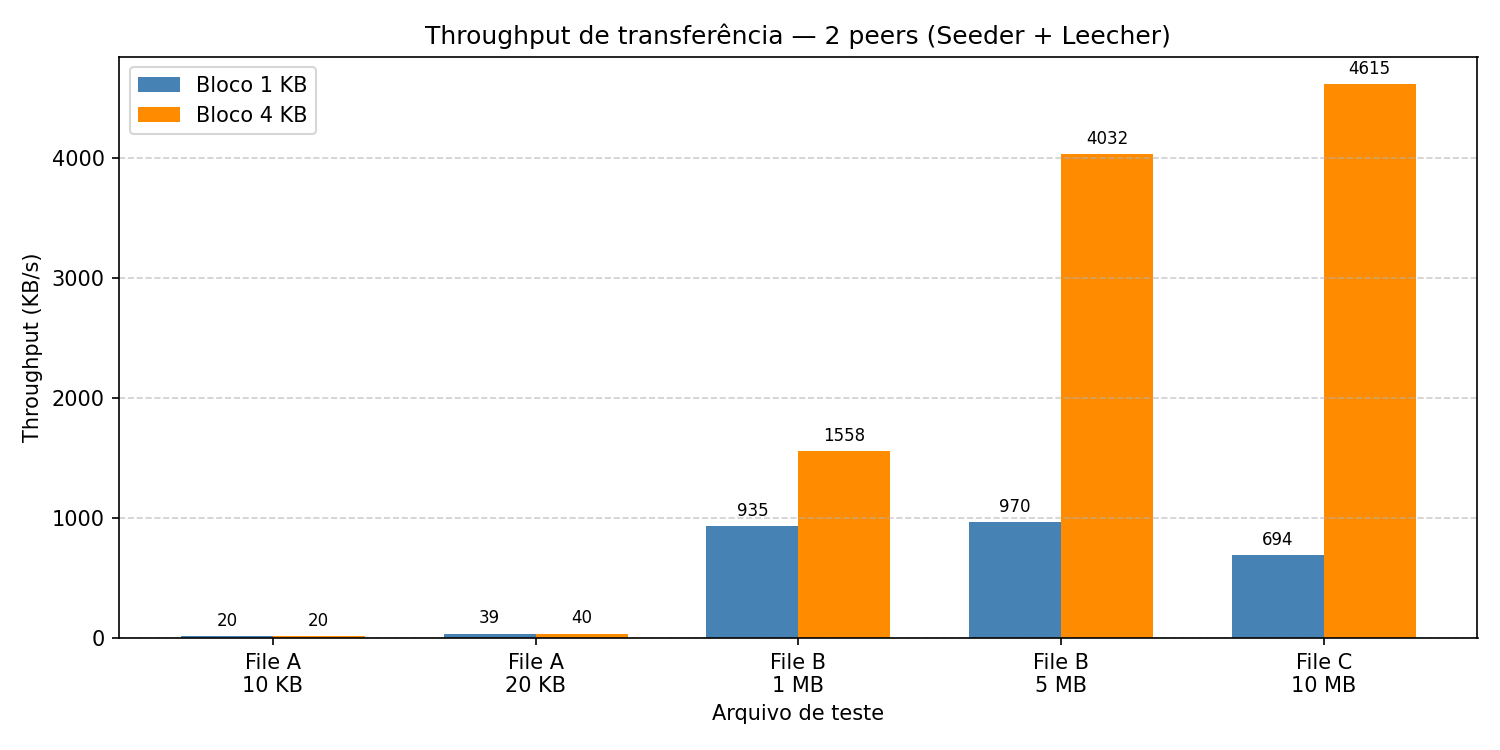
\includegraphics[width=0.95\linewidth]{throughput.png}
    \caption{Throughput de transferência por arquivo e tamanho de bloco (2 peers).}
    \label{fig:throughput}
\end{figure}

\begin{figure}[H]
    \centering
    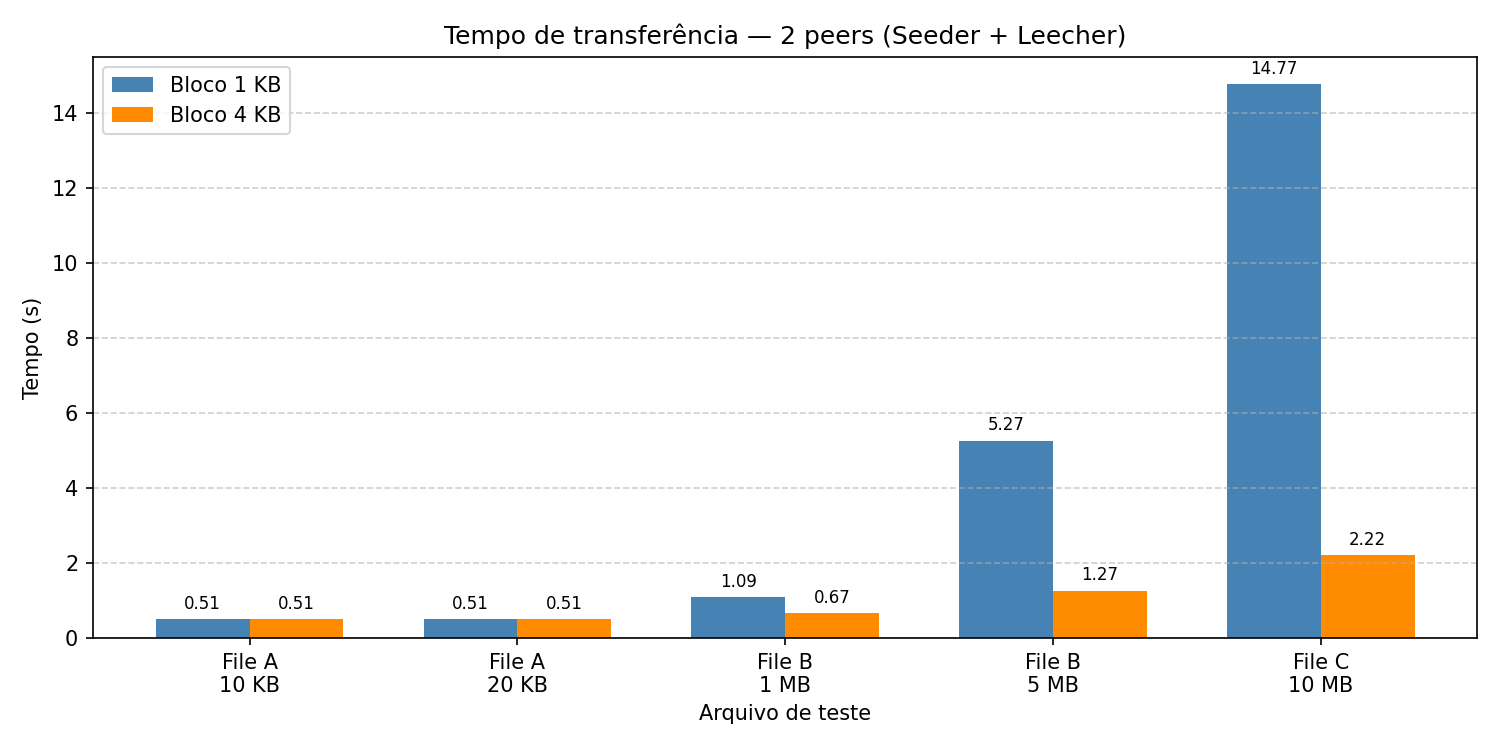
\includegraphics[width=0.95\linewidth]{tempo.png}
    \caption{Tempo de transferência por arquivo e tamanho de bloco (2 peers).}
    \label{fig:tempo}
\end{figure}

\begin{figure}[H]
    \centering
    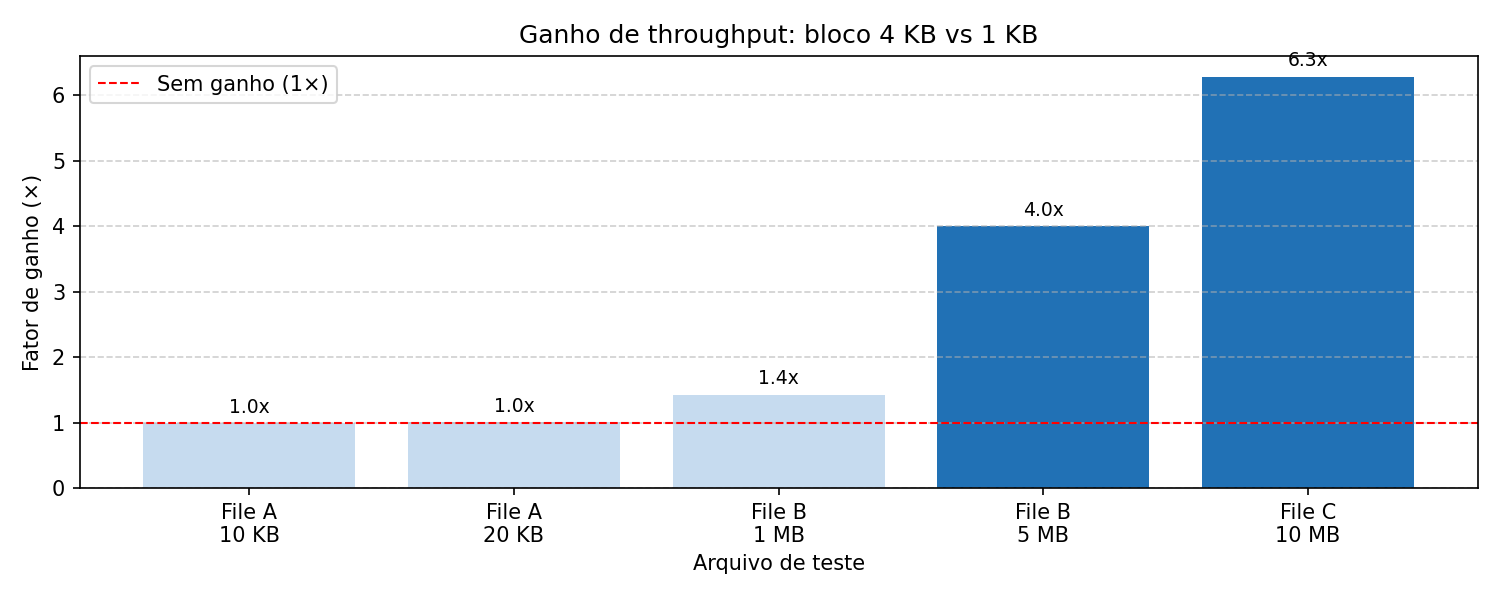
\includegraphics[width=0.95\linewidth]{ganho.png}
    \caption{Fator de ganho de throughput ao usar blocos de 4 KB em vez de 1 KB.}
    \label{fig:ganho}
\end{figure}

\subsection{Análise}

\paragraph{Impacto do tamanho do bloco.}
Blocos maiores (4\,KB vs 1\,KB) reduzem o número de round-trips TCP e o
overhead de headers, resultando em throughput significativamente superior para
arquivos médios e grandes. Com conexões persistentes, o ganho é evidente:
$\approx 1{,}80$\,MB/s com 4\,KB contra $\approx 1{,}26$\,MB/s com 1\,KB
no File B de 1\,MB (ganho $\approx 1{,}43\times$), e
$\approx 6{,}51$\,MB/s contra $\approx 1{,}04$\,MB/s no File C de 10\,MB
(ganho $\approx 6{,}29\times$). Para arquivos pequenos (10--20\,KB) o
impacto é desprezível, pois o overhead de conexão domina o tempo total.

\paragraph{Impacto do número de peers.}
Com 4 peers, C e D conectam-se a A e a B, podendo aproveitar os blocos
que B já recebeu. Para o File C (10\,MB) com bloco de 4\,KB, o seeder
ainda estava ativo quando C e D iniciaram, de modo que os três leechers
concluíram em $\approx 2$\,s com throughput entre 4,6 e 5,2\,MB/s.
Para arquivos pequenos (File A/B com 4\,KB de bloco), B conclui e encerra
o processo antes que C e D consigam conectar-se a ele, forçando-os a usar
apenas A como fonte; as cinco tentativas de reconexão (0,5\,s cada)
explicam o tempo de $\approx 3$\,s para esses casos.
O servidor não-bloqueante baseado em \texttt{select()} atendeu múltiplos
leechers simultâneos com um único loop de eventos, sem degradação
perceptível para o File C.

\paragraph{Integridade.}
Todos os 16 cenários testados produziram SHA-256 idêntico ao original,
confirmando que o protocolo garante integridade mesmo sob acesso concorrente
ao buffer de blocos e com múltiplos leechers simultâneos.

% -------------------------------------------------------
\section{Conclusão}

A implementação demonstra os princípios centrais do modelo P2P: simetria
(cada peer serve e consome simultaneamente), fragmentação de arquivos e
remontagem verificada por hash. O protocolo binário simples mostrou-se
suficiente para transferências confiáveis em rede local. Como evolução
natural, conexões persistentes por peer (em vez de uma por bloco) e
estratégias de seleção de blocos mais inteligentes (\emph{rarest-first})
aumentariam o throughput em redes com maior latência.

\end{document}
